\documentclass[11pt,a4paper]{article}
\usepackage[T1]{fontenc}
\usepackage[margin=2.3cm]{geometry}
\usepackage{amsmath,amssymb}
\usepackage{graphicx}
\usepackage[dvipsnames]{xcolor}
\usepackage{enumitem}
\usepackage[colorlinks=true,linkcolor=blue,urlcolor=blue]{hyperref}
\setlength{\parskip}{0.6em}
\setlength{\parindent}{0pt}
\begin{document}

\begin{center}{\LARGE\bfseries openohm}\\[0.4em]{\large Ohm's law to a safe resistor design, in three sessions.}\\[0.2em]\small PAN IIT OSS explainer \textbullet{} secondary school to diploma / undergraduate (levels 3-5)\end{center}

\section*{Why this exists}
Every electronic device is a set of parts that share a voltage and a current. This explainer shows the mathematics of the simplest circuit law, Ohm's law, and of the heat it produces, using only algebra and a small amount of numerical solving, so you can build it yourself.

\section*{The end goal}
Design a resistor circuit to a power and current limit with Ohm's law. The end goal is to design a resistor circuit to a current and a power limit with Ohm's law. The same reasoning scales from a hobby LED to the cabling of a machine, but only as a simplified low-voltage educational model: never design mains installations from it.

\section*{How the three sessions build up}
\begin{enumerate}[nosep]
\item \textbf{Session 1: Ohm's law and electrical power} (Level 1, conceptual interactive model, 60 min).
\item \textbf{Session 2: Resistor networks, power ratings and a design to a limit} (Level 2, mathematical engineering model, 75 min).
\item \textbf{Session 3: A non-ohmic LED: solve it numerically and validate} (Level 3, simulation and validation, 90 min).
\end{enumerate}

\section{Session 1: Ohm's law and electrical power}

\subsection*{A. Real-world problem}
A phone charger, a torch bulb and a kettle each push electric current through something that resists it. Why does a thin wire get hot while a thick one does not, and why does a small resistor burn out if you connect it to too large a battery? Two short rules answer both: Ohm's law tells you how much current flows, and the power formula tells you how much heat appears. This repo uses low-voltage circuits only (batteries and small supplies, never mains).

\subsection*{B. Concept and theory}
Voltage V is the electrical push between two points. Resistance R is how strongly a part resists the flow. Current I is the flow of charge. For an ohmic part (one whose R stays constant) the three are linked by Ohm's law. The resistor turns electrical energy into heat at a rate called power, P = V I. Substituting Ohm's law gives two more forms that are often easier to use: P = I\textasciicircum{}2 R when you know the current, and P = V\textasciicircum{}2 / R when you know the voltage.

\begin{itemize}[nosep]
\item V: voltage across the resistor (V (volts))
\item I: current through the resistor (A (amperes))
\item R: resistance (ohm)
\item P: power turned into heat (W (watts))
\end{itemize}

\begin{equation*}
V = I\,R \quad\Longleftrightarrow\quad I = \frac{V}{R}
\end{equation*}

\begin{equation*}
P = V\,I
\end{equation*}

\begin{equation*}
P = I^2 R = \frac{V^2}{R}
\end{equation*}

\begin{center}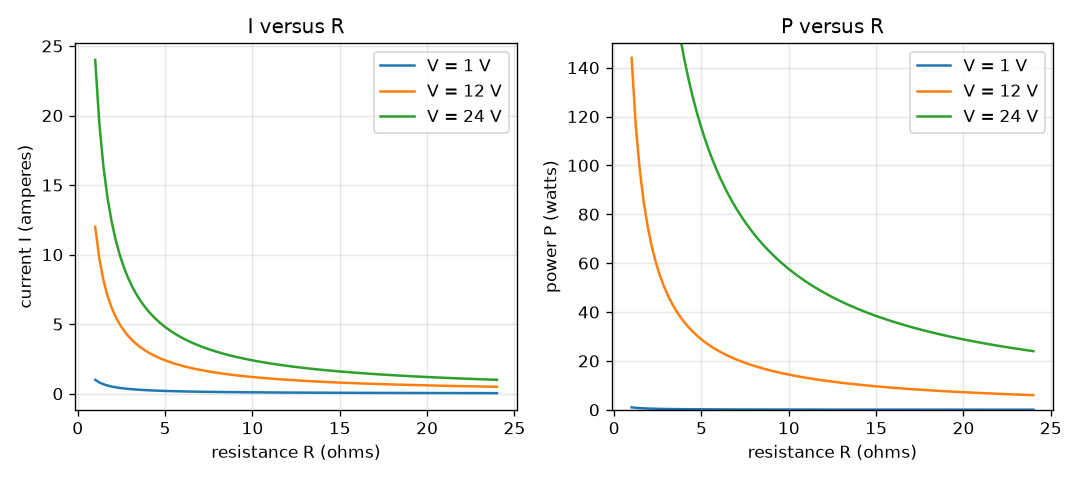
\includegraphics[width=0.85\linewidth]{figures/s01_i_p_vs_r.png}\\\small Current and power against resistance at 1, 12 and 24 V: both fall as 1/R.\end{center}

\subsection*{E. Worked example}
A 12 V supply is connected across a 6 ohm resistor. Find the current and the power, and check the power in all three forms.
\begin{enumerate}[nosep]
\item I = V / R = 12 V / 6 ohm = 2 A.
\item P = V I = 12 V x 2 A = 24 W.
\item Check with I\textasciicircum{}2 R = 2\textasciicircum{}2 x 6 = 4 x 6 = 24 W.
\item Check with V\textasciicircum{}2 / R = 144 / 6 = 24 W. All three forms agree.
\end{enumerate}
\textbf{Answer.} The current is 2 A and the resistor dissipates 24 W.

\subsection*{F. Questions}
\begin{enumerate}[nosep]
\item \textbf{Conceptual.} If you double the voltage across a resistor, what happens to the current and to the power? Explain why they change by different factors.
\item \textbf{Numerical.} What current does a 24 ohm resistor draw from an ideal 12 V supply, and how much power does it dissipate? Do a sanity check.
\item \textbf{Graph and simulation interpretation.} On the P versus R graph at 12 V, what is P at 6, 12 and 24 ohm? What does the pattern tell you about halving the resistance?
\item \textbf{Design and optimisation challenge.} Design: from the preset resistors 1, 6, 12 and 24 ohm, choose one for a 12 V supply so that the current is at most 1 A and the resistor dissipates at most 10 W. What is the smallest resistance, not limited to presets, that meets both limits?
\end{enumerate}

\section{Session 2: Resistor networks, power ratings and a design to a limit}

\subsection*{A. Real-world problem}
You have a 12 V supply, a bag of small resistors, each rated 0.25 W, and you want about 0.1 A to flow. One 120 ohm resistor would carry the right current but would try to dissipate 1.2 W, nearly five times its rating, and it would overheat. Can several resistors share the job safely, and what is the fewest you need? (Low-voltage educational model: never design mains equipment this way.)

\subsection*{B. Concept and theory}
In series (one path) the same current flows through every resistor and the resistances add. In parallel (several paths between the same two points) every branch has the same voltage and the conductances (1/R) add, so the total is smaller than the smallest branch. Once the total resistance is known, Ohm's law gives the total current. The current then splits among parallel branches, and each resistor's power is I\textasciicircum{}2 R with its own current. A grid of ns resistors in series per branch and np branches in parallel, each of value r, has total R = ns r / np, and each resistor carries I / np. Every part has a power rating, the largest power it can dissipate continuously.

\begin{itemize}[nosep]
\item R\_total: equivalent resistance of the network (ohm)
\item ns: resistors in series in each branch (no unit)
\item np: branches in parallel (no unit)
\item r: value of each resistor (ohm)
\item P\_each: power in each resistor (W)
\item rating: largest allowed power per resistor (0.25 W here) (W)
\end{itemize}

\begin{equation*}
R_{\mathrm{series}} = R_1 + R_2 + \dots
\end{equation*}

\begin{equation*}
\frac{1}{R_{\mathrm{parallel}}} = \frac{1}{R_1} + \frac{1}{R_2} + \dots
\end{equation*}

\begin{equation*}
R_{\mathrm{total}} = \frac{n_s\, r}{n_p},\qquad I = \frac{V}{R_{\mathrm{total}}},\qquad P_{\mathrm{each}} = \left(\frac{I}{n_p}\right)^2 r
\end{equation*}

\begin{center}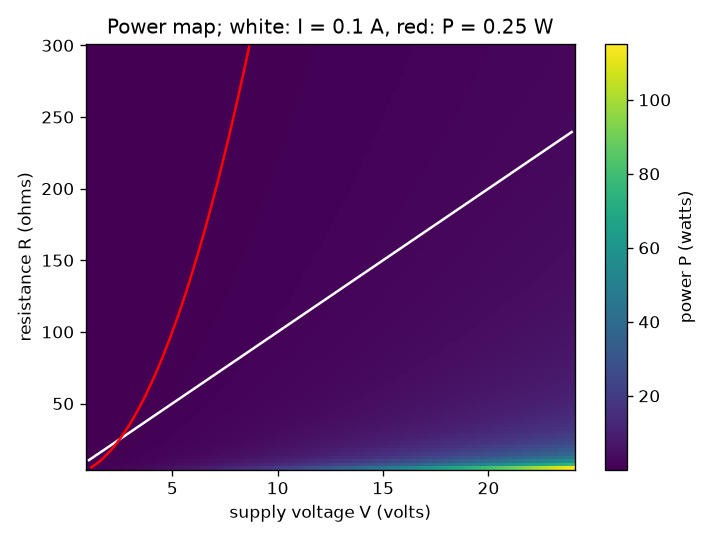
\includegraphics[width=0.85\linewidth]{figures/s02_design_map.png}\\\small Power against supply voltage and total resistance; white: 0.1 A, red: 0.25 W.\end{center}

\subsection*{E. Worked example}
A 12 V supply feeds a grid of six 180 ohm resistors: two in series per branch, three branches in parallel. Find the total resistance, the current, and the power in each resistor.
\begin{enumerate}[nosep]
\item One branch is two resistors in series: 180 + 180 = 360 ohm.
\item Three equal 360 ohm branches in parallel: R\_total = 360 / 3 = 120 ohm.
\item Total current I = 12 / 120 = 0.1 A.
\item Each branch carries 0.1 / 3 = 0.0333 A.
\item Power in each resistor = (0.0333)\textasciicircum{}2 x 180 = 0.200 W, below the 0.25 W rating.
\item Check: six resistors x 0.2 W = 1.2 W = V I = 12 x 0.1. The powers add up.
\end{enumerate}
\textbf{Answer.} R\_total = 120 ohm, I = 0.1 A, each resistor 0.200 W (total 1.2 W).

\subsection*{F. Questions}
\begin{enumerate}[nosep]
\item \textbf{Conceptual.} Why does adding a resistor in parallel make the total resistance smaller, even though you added more material?
\item \textbf{Numerical.} A 12 V supply feeds a 6 ohm resistor in series with two 12 ohm resistors in parallel. Find the total current, the power in the 6 ohm resistor and the power in each 12 ohm resistor.
\item \textbf{Graph and simulation interpretation.} In the power graph for a single 120 ohm resistor, at what supply voltage does the curve cross the 0.25 W rating? Where does it cross for the 2 x 3 grid of 180 ohm resistors?
\item \textbf{Design and optimisation challenge.} Design: with a 12 V supply and 0.25 W resistors, get 50 mA within 5 percent using the fewest E12 resistors. State the network and its checks.
\end{enumerate}

\section{Session 3: A non-ohmic LED: solve it numerically and validate}

\subsection*{A. Real-world problem}
Connect an LED straight to a battery and it burns out in a flash. An LED is not a resistor: below about 1.5 V almost no current flows, and just above it the current climbs steeply. A series resistor limits the current. But what current actually flows, and how much does it change if the supply is 10 percent off? Ohm's law alone cannot say, because the LED has no single resistance. (Simplified low-voltage model, not a datasheet; never use it for mains.)

\subsection*{B. Concept and theory}
An LED follows an exponential current-voltage law, I = I\_s (exp(Vd / N\_VT) - 1), where I\_s is a tiny saturation current and N\_VT sets how sharp the turn-on is. Here the model is tuned so that 20 mA gives 2.0 V. In series with a resistor R on a supply Vs, Kirchhoff's voltage law says Vs = I R + Vd. Substituting the LED law gives one equation in Vd that has no neat algebraic solution, so we solve it numerically. Newton's method improves a guess by following the tangent: Vd\_new = Vd - f / f'. Bisection halves a bracket that contains the root and is slow but safe, so it serves as a reference. A small change dVs in the supply changes the current by dI = dVs / (R + r\_d), where r\_d = N\_VT / I is the LED's dynamic resistance, the slope of its curve at the operating point.

\begin{itemize}[nosep]
\item Vs: supply voltage (V)
\item R: series resistor (ohm)
\item Vd: voltage across the LED (V)
\item I: loop current (A)
\item I\_s: saturation current of the model (A)
\item N\_VT: ideality factor times thermal voltage (0.05 here) (V)
\item r\_d: dynamic resistance of the LED, N\_VT / I (ohm)
\end{itemize}

\begin{equation*}
I = I_s\left(e^{V_d/N_{VT}} - 1\right)
\end{equation*}

\begin{equation*}
V_s = I R + V_d \;\;\Rightarrow\;\; f(V_d) = I_s\left(e^{V_d/N_{VT}} - 1\right) - \frac{V_s - V_d}{R} = 0
\end{equation*}

\begin{equation*}
V_d \leftarrow V_d - \frac{f(V_d)}{f'(V_d)},\qquad f'(V_d) = \frac{I_s}{N_{VT}}e^{V_d/N_{VT}} + \frac{1}{R}
\end{equation*}

\begin{equation*}
\frac{dI}{dV_s} = \frac{1}{R + r_d},\qquad r_d = \frac{N_{VT}}{I}
\end{equation*}

\begin{center}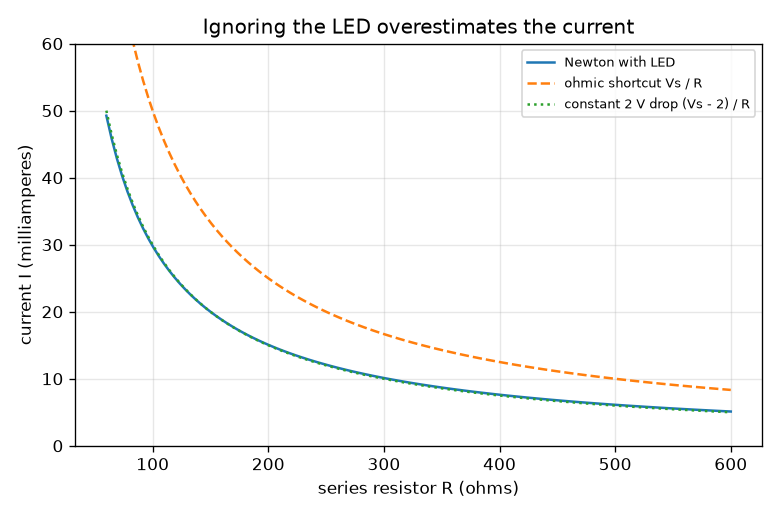
\includegraphics[width=0.85\linewidth]{figures/s03_led_current_vs_r.png}\\\small Current against series resistance: the ohmic shortcut overestimates, a constant 2 V drop is close.\end{center}

\subsection*{E. Worked example}
A 5 V supply feeds a 150 ohm resistor in series with the LED. Find the operating point, check it against Kirchhoff's law, and compare with the ohmic shortcut.
\begin{enumerate}[nosep]
\item Guess that the LED drops about 2.0 V (the tuned point). The resistor then has 5 - 2 = 3 V across it.
\item I = 3 / 150 = 0.020 A = 20 mA, which is exactly the current at which the model gives 2.0 V, so the guess is consistent.
\item Newton's method started from 2.5 V reaches Vd = 2.000 V, I = 20.00 mA in 16 steps; bisection gives the same values.
\item Kirchhoff check: I R + Vd = 0.020 x 150 + 2.0 = 5.0 V = Vs.
\item Powers: resistor 0.020\textasciicircum{}2 x 150 = 0.060 W, LED 2.0 x 0.020 = 0.040 W, total 0.100 W = 5 x 0.02.
\item The ohmic shortcut Vs / R = 5 / 150 = 33.3 mA is 67 percent too high, because it ignores the 2 V that the LED takes.
\end{enumerate}
\textbf{Answer.} Operating point: Vd = 2.000 V, I = 20.0 mA; resistor 60 mW, LED 40 mW. Ignoring the LED would give 33.3 mA.

\subsection*{F. Questions}
\begin{enumerate}[nosep]
\item \textbf{Conceptual.} Why does an LED need a series resistor, but an ordinary resistor does not?
\item \textbf{Numerical.} For Vs = 5 V and R = 150 ohm use the sensitivity formula to estimate how much the LED current changes if the supply rises by 0.5 V. Compare with the value from the model (23.3 mA at 5.5 V).
\item \textbf{Graph and simulation interpretation.} In the load-line figure the three operating points have LED voltages between 1.99 and 2.01 V but currents between 16.7 and 23.3 mA. What does that say about which part controls the current?
\item \textbf{Design and optimisation challenge.} Design: a 5 V supply (4.5 to 5.5 V) must give 10 to 25 mA in the LED and use at most 0.12 W in total at 5.5 V. Choose from the E12 series and justify.
\end{enumerate}

\section{Real-world mini-project}
\textbf{Design a safe LED indicator within a power budget.} A 5 V supply is only guaranteed to within 10 percent (4.5 to 5.5 V). A red LED must stay visible (at least 10 mA) but never exceed its 25 mA limit, and the whole circuit may use at most 0.12 W at the highest supply voltage. Choose a standard E12 series resistor using \texttt{pick\_resistor} and \texttt{solve\_newton} from Session 3. This is general education about a simplified LED model, not a datasheet-based design.

\section{The path ahead}
\begin{enumerate}[nosep]
\item \textbf{Session 4: Network synthesis for any target.} A function that, for any target resistance from 10 to 1000 ohm, returns the best network of at most two different E12 resistors.
\item \textbf{Session 5: Self-heating resistor.} A heater model R(T) = R0 (1 + alpha (T - T0)) with a thermal resistance to the surroundings.
\item \textbf{Session 6: Tolerance and Monte Carlo.} A Monte Carlo run of the 2 x 3 grid with random resistor values.
\item \textbf{Session 7: Real battery and maximum power transfer.} A battery with internal resistance r feeding a load R, with the power in the load swept over R.
\item \textbf{Session 8: Add a capacitor: the RC time constant.} A numerical step response of a resistor and capacitor in series.
\end{enumerate}

\section{Answers and hints}

\subsection*{Session 1}
\begin{enumerate}[nosep]
\item \textbf{Conceptual.} Hint: Use I = V / R first, then P = V I with the new current. Solution: The current doubles because I = V / R is proportional to V. The power is V times I, and both doubled, so P rises by 2 x 2 = 4 (also V\textasciicircum{}2 / R: V\textasciicircum{}2 quadruples). Power depends on voltage twice: once because the push is larger, once because the flow is larger.
\item \textbf{Numerical.} Hint: I = V / R, then P = V I. Solution: I = 12 / 24 = 0.5 A and P = 12 x 0.5 = 6 W. Sanity check: the 6 ohm resistor of the worked example drew 2 A, and this resistor is four times larger, so the current should be four times smaller: 2 / 4 = 0.5 A. Units: volts divided by ohms gives amperes; volts times amperes gives watts.
\item \textbf{Graph and simulation interpretation.} Hint: Read the dot for each resistor, or use P = V\textasciicircum{}2 / R = 144 / R. Solution: P = 24 W at 6 ohm, 12 W at 12 ohm and 6 W at 24 ohm. Each time R is halved, P doubles, because P = 144 / R is inversely proportional to R at fixed voltage. Cutting the resistance of a part on a fixed supply makes it hotter, not cooler.
\item \textbf{Design and optimisation challenge.} Hint: Each limit gives a minimum R: R \textgreater{}= V / I\_max and R \textgreater{}= V\textasciicircum{}2 / P\_max. Solution: Current limit: R \textgreater{}= 12 / 1 = 12 ohm. Power limit: R \textgreater{}= 144 / 10 = 14.4 ohm. Both must hold, so R \textgreater{}= 14.4 ohm. Among the presets only 24 ohm qualifies (12 ohm gives exactly 1 A but 12 W, over 10 W). The 24 ohm choice gives 0.5 A and 6 W. Trade-off: a larger R is safer but delivers less current to the load.
\end{enumerate}

\subsection*{Session 2}
\begin{enumerate}[nosep]
\item \textbf{Conceptual.} Hint: Think of the number of paths the current can take. Solution: A parallel resistor opens one more path for the current. With every branch at the same voltage, each branch carries its own current and the total current is the sum, so for the same voltage the total current rises and the equivalent resistance V / I falls. It is always smaller than the smallest branch.
\item \textbf{Numerical.} Hint: First combine the two 12 ohm resistors, then add the 6 ohm resistor. Solution: Two 12 ohm resistors in parallel give 6 ohm. In series with 6 ohm: R\_total = 12 ohm, so I = 12 / 12 = 1 A. The 6 ohm resistor carries 1 A: P = 1\textasciicircum{}2 x 6 = 6 W. The current splits equally, 0.5 A in each 12 ohm resistor: P = 0.5\textasciicircum{}2 x 12 = 3 W each. Check: 6 + 3 + 3 = 12 W = 12 V x 1 A.
\item \textbf{Graph and simulation interpretation.} Hint: Solve V\textasciicircum{}2 / R = 0.25 for the single resistor; for the grid, P\_each = (V / 120 / 3)\textasciicircum{}2 x 180. Solution: Single resistor: V = sqrt(0.25 x 120) = sqrt(30) = 5.48 V. Grid: P\_each = V\textasciicircum{}2 x 180 / 129600 = V\textasciicircum{}2 / 720, which equals 0.25 at V = sqrt(180) = 13.4 V. So the grid is safe at 12 V, but only with about 1.4 V of margin.
\item \textbf{Design and optimisation challenge.} Hint: Target R\_total is 240 ohm. One resistor would dissipate 0.6 W. Try series chains of identical E12 values. Solution: Three 82 ohm resistors in series give 246 ohm: I = 12 / 246 = 48.8 mA (2.4 percent low, inside 5 percent), each resistor dissipates 0.0488\textasciicircum{}2 x 82 = 0.195 W, below 0.25 W. One or two resistors cannot meet the power rating at 50 mA. Trade-off: more parts cost more and take space; the margin is 22 percent below the rating. Assumption: tolerance of the parts is ignored.
\end{enumerate}

\subsection*{Session 3}
\begin{enumerate}[nosep]
\item \textbf{Conceptual.} Hint: Compare how the current changes when the voltage across each rises by a small amount. Solution: For a resistor the current rises in proportion to the voltage, gently. For an LED the current rises exponentially: a few hundredths of a volt more across the LED can multiply the current several times, so any small error in the supply would destroy it. The series resistor takes most of the extra voltage and fixes the current to roughly (Vs - Vd) / R.
\item \textbf{Numerical.} Hint: dI/dVs = 1 / (R + N\_VT / I) with I = 20 mA and N\_VT = 0.05 V. Solution: r\_d = 0.05 / 0.020 = 2.5 ohm, so dI/dVs = 1 / 152.5 = 6.56 mA per volt. For 0.5 V: change = 3.3 mA, estimate 23.3 mA. The model gives 23.28 mA, so they agree. The tiny r\_d means the resistor, not the LED, sets the sensitivity: dI/dVs is almost 1 / R.
\item \textbf{Graph and simulation interpretation.} Hint: Look at the vertical spread of the dots against their horizontal spread. Solution: The LED curve is almost vertical there, so the LED voltage is nearly fixed (about 2 V) and the load line decides where the point sits along it: the resistor and the supply set the current. This is why designers use I = (Vs - Vd) / R with a fixed Vd of about 2 V.
\item \textbf{Design and optimisation challenge.} Hint: Run pick\_resistor(5.0, 0.10, 0.010, 0.025, 0.12) and look at the current range for each choice. Solution: The safe E12 values are 180 and 220 ohm. 150 ohm gives up to 23.3 mA but 0.128 W at 5.5 V, over budget; 270 ohm falls to 9.4 mA at 4.5 V, too dim. For 180 ohm the current is 14.0 to 19.4 mA and the total power at 5.5 V is 0.107 W; for 220 ohm it is 11.5 to 16.0 mA and 0.088 W. Choose 180 ohm for brightness or 220 ohm for the smaller power; both leave the 0.25 W resistor far below its rating. Assumption: a tolerance of the resistor itself is ignored (5 percent changes these numbers a little).
\end{enumerate}

\section{How to join}
Read \texttt{CONTRIBUTING.md} in the repository, then pick an issue labelled \texttt{good first issue}. Repository: \url{https://github.com/KrunalPanchal1995/openohm}

\end{document}
